\graphicspath{{images/}}

\section{Ход работы}

Я выбрал набор данных Rice type classification \cite{kaggle} для выполнения лабораторной работы. Требуется предсказать, 
какой тип риса представлен (Jasmine - 1, Gonen - 0), основываясь на его признаках (таких как площадь, средняя ширина и длина, скругленность и т.д.).

Признаки в наборе данных:

\begin{enumerate}
    \item
    Id --- номер риса, данный столбец из данных был удалён (очевидно, что номер входных данных признаков не влияет на результат).
    \item
    Area --- регион выращивания риса.
    \item
    MajorAxisLength --- результат измерения длины риса.
    \item
    MinorAxisLength --- результат ширины риса.
    \item
    Eccentricity --- степень отклонения контура риса от окружности.
    \item
    ConvexArea --- площадь выпуклой поверхности риса.
    \item
    EquivDiameter --- диаметр сферы, эквивалентной по объёму рису.
    \item
    Extent --- площадь риса.
    \item
    Perimeter --- периметр контура риса.
    \item
    Roundness --- коэффициент "скругленности" контура риса.
    \item
    AspectRation --- соотношение длины и ширины риса.
    \item
    Class --- Тип риса.
\end{enumerate}

Перед выявлением зависимостей между признаками следует проверяю целостность набора данных:
\begin{alltt}
RangeIndex: 18185 entries, 0 to 18184
Data columns (total 11 columns):
 #   Column           Non-Null Count  Dtype  
---  ------           --------------  -----  
 0   Area             18185 non-null  int64  
 1   MajorAxisLength  18185 non-null  float64
 2   MinorAxisLength  18185 non-null  float64
 3   Eccentricity     18185 non-null  float64
 4   ConvexArea       18185 non-null  int64  
 5   EquivDiameter    18185 non-null  float64
 6   Extent           18185 non-null  float64
 7   Perimeter        18185 non-null  float64
 8   Roundness        18185 non-null  float64
 9   AspectRation     18185 non-null  float64
 10  Class            18185 non-null  int64  
dtypes: float64(8), int64(3)
memory usage: 1.5 MB
\end{alltt}

В наборе нет неполных данных, а все признаки - числовые.
\pagebreak

Построю графики для каждой пары признаков. Синим отмечен рис типа Jasmin, оранжевым - Gonen:
\begin{center}
\includegraphics[scale=0.25]{pair0}
\end{center}\pagebreak

Построю корреляционную матрицу для признаков:
\begin{center}
\includegraphics[scale=0.65]{corr0}
\end{center}
Так же построю гистограммы для числовых признаков:
\begin{center}
\includegraphics[scale=0.35]{bar0}
\end{center}
Имеется небольшое количество выбросов у некоторых признаков. Удалю все данные, где Roundness < 0.5, Perimeter > 420 и Eccentricity < 0.85 
\pagebreak

Теперь ничего не мешает анализу. Построю те же графики для обработанного набора данных:
\begin{center}
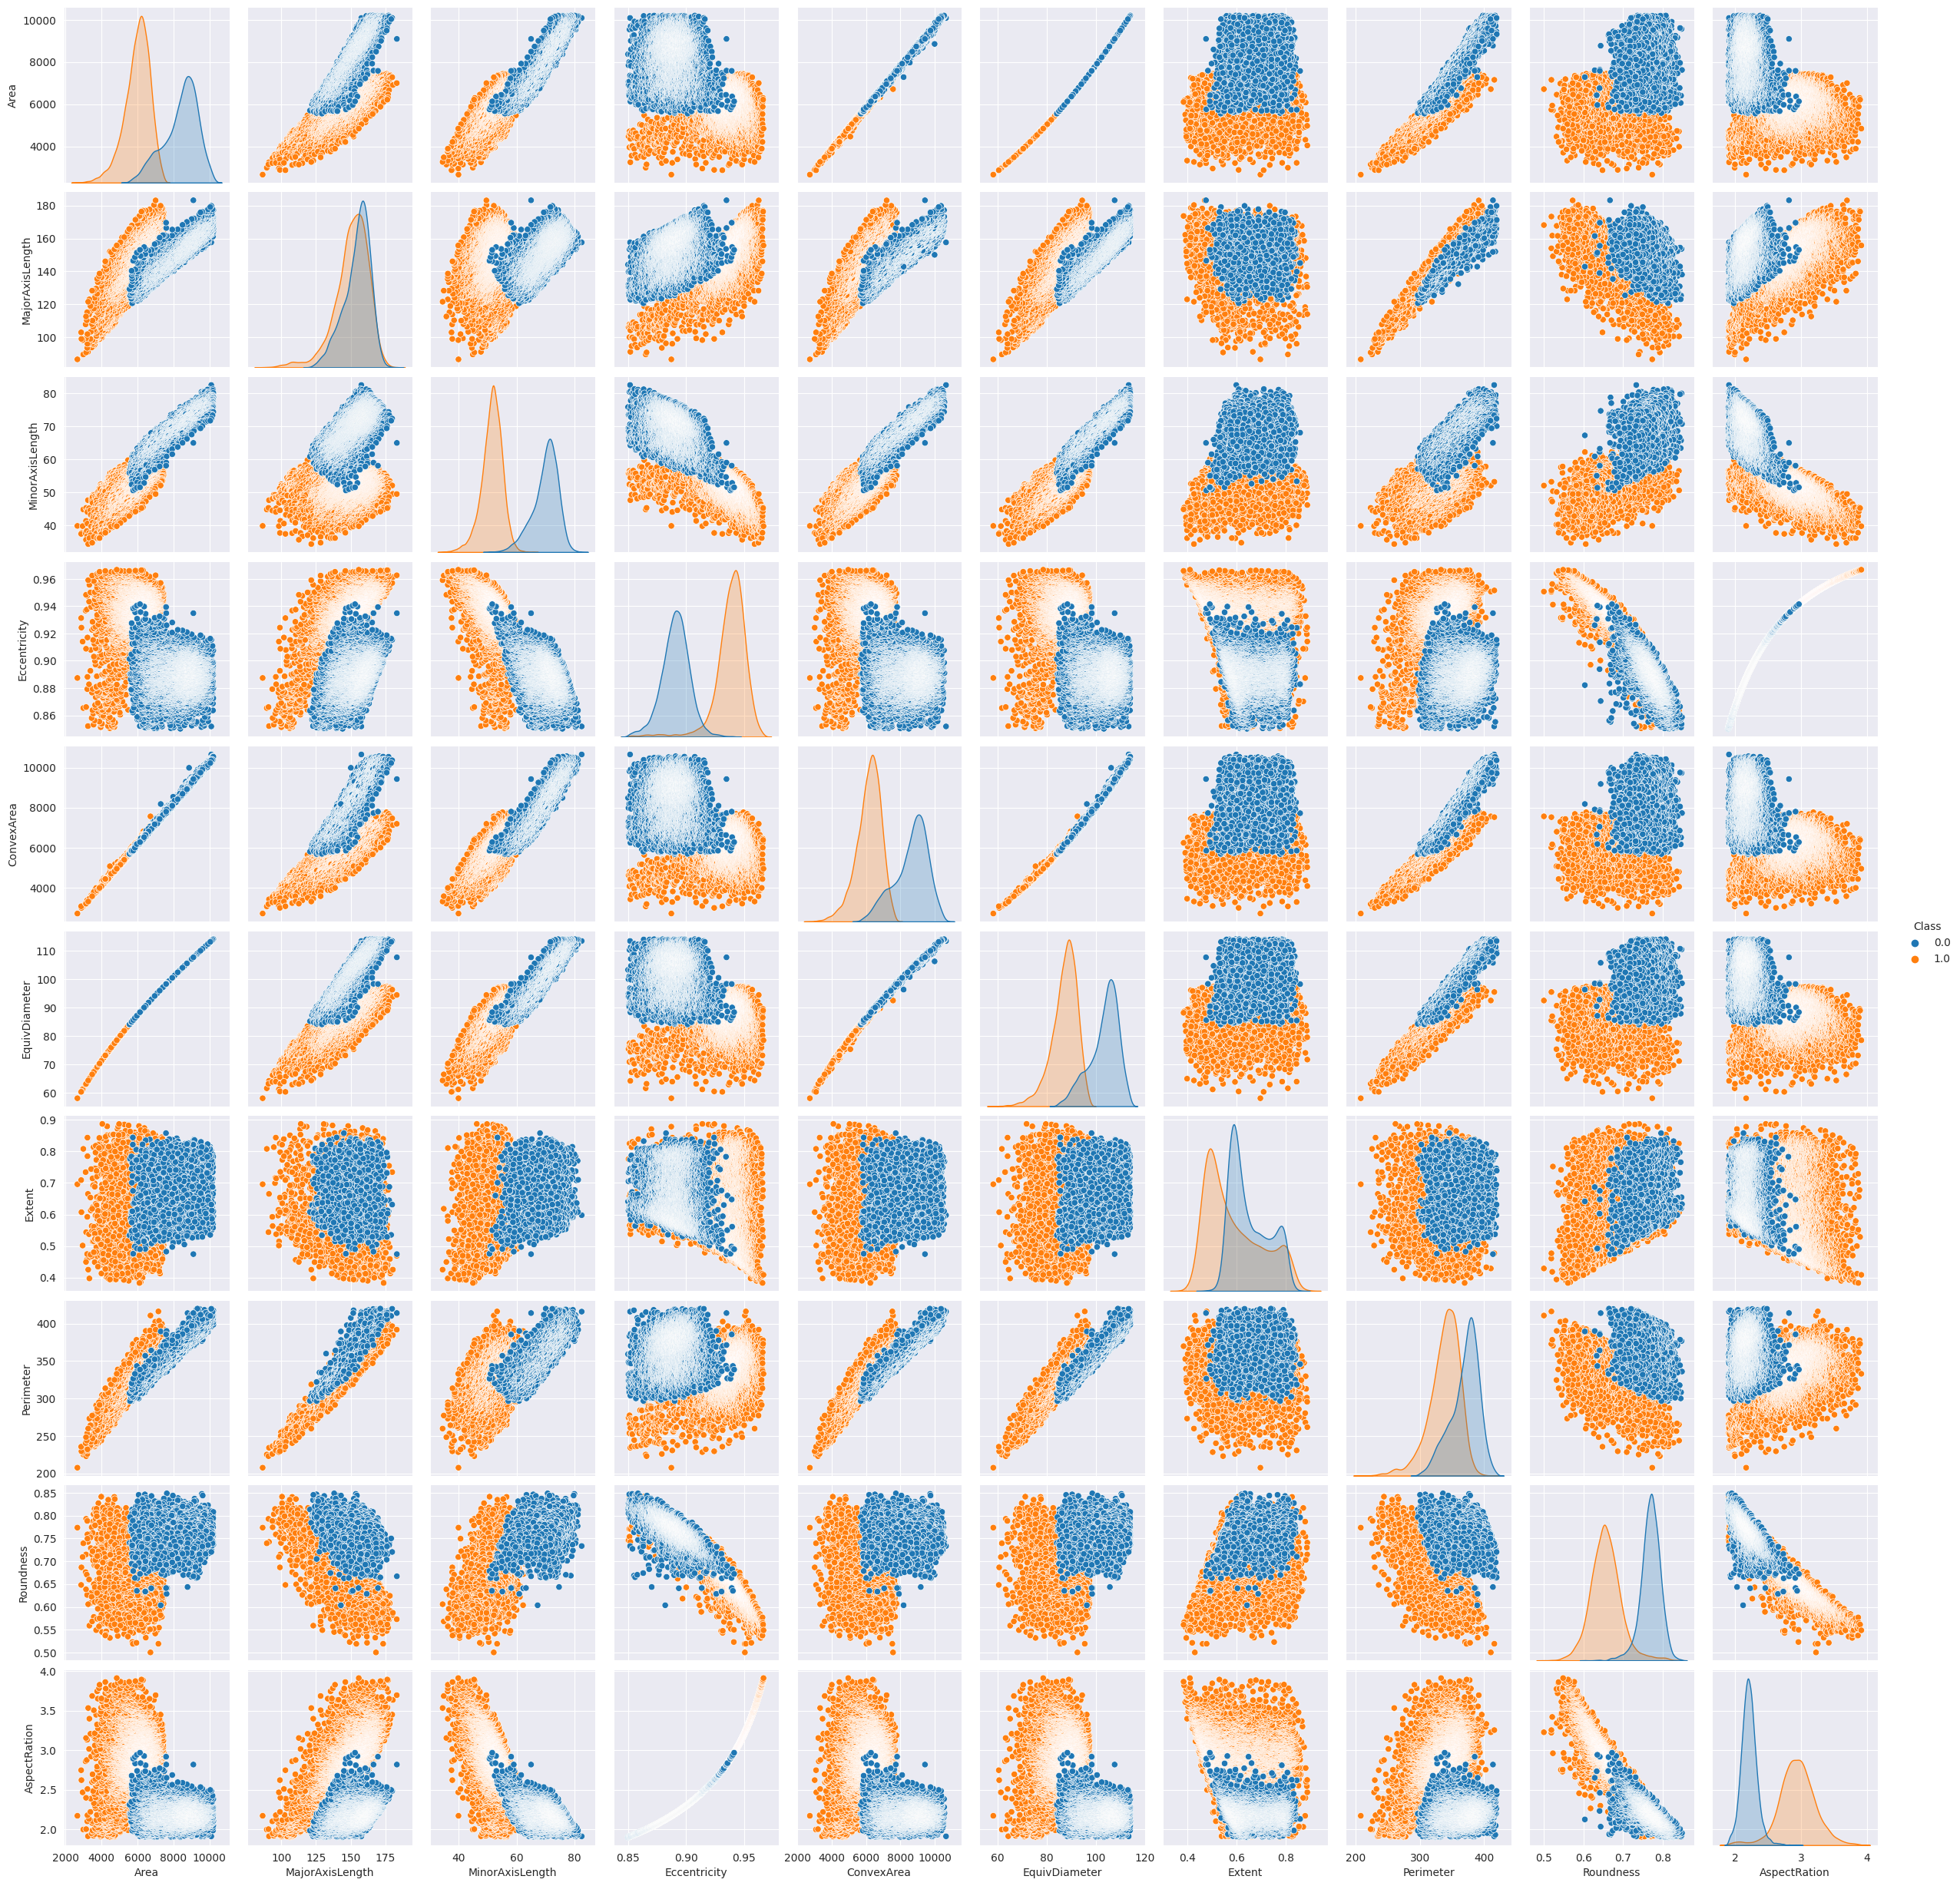
\includegraphics[scale=0.25]{pair1}
\end{center}
Исходя из парных графиков, можно сделать вывод, что задачу реально решить линейной моделью. Однако, на некоторой части графиков не представляется
возможным провести точную прямую линию, которая бы разделяла два класса, а признак MajorAxisLength вообще практически не коррелирует с целевым классом,
что отчётливо заметно на одном из диагональных графиков.
\pagebreak

Корреляционная матрица после удаления выбросов не изменилась:
\begin{center}
\includegraphics[scale=0.65]{corr1}
\end{center}
Видно, что почти все признаки, кроме <<MajorAxisLength>>, <<Extent>> и <<Perimeter>>, очень сильно влияют на конечный результат. Также некоторые признаки
довольно сильно коррелируют между собой, что может быть объяснено тем, что всё это, по сути, геометрические параметры, которые связаны между собой, т.к. контур
риса обоих сортов напоминает эллипс.

Гистограммы распределения числовых признаков:
\begin{center}
\includegraphics[scale=0.35]{bar1}
\end{center}
Полученных данных достаточно для построения модели, об этом говорят попарные графики и корреляционная матрица. Добавление новых признаков не требуется.

\pagebreak

Соотношение классов объектов:
\begin{center}
\includegraphics[scale=0.65]{classes}
\end{center}
Объектов разных классов примерно одинаковое количество, oversampling не требуется. Данные готовы к обучению.

\pagebreak
